% !TEX root = ../main.tex

\section{Exploratory Analysis and Examples} \label{sec:analysis}

In this section, we provide examples and use-cases on the dataset. Code to
reproduce our examples is available online, in the \texttt{examples} folder.

\subsection{Visualizations}

\paragraph{Roster.}
%The file \texttt{roster.csv} contains information about $N=35{,}430$ CPD
%officers. For each officer --- identified by a Unique Identifier (``uid''),
%\texttt{roster.csv} provides, among other covariates, the officer's name,
%gender, race, birthyear, appointment and resignation dates. It is
%straightforward  to use the data to generate summary statistics, e.g., using
%appointment and resignation dates to understand the number of appointments,
%retirements as well as active officers over the years of  (\Cref{fig:history}).
%We report in \Cref{tab:stats} some 


\begin{figure}[t!] 
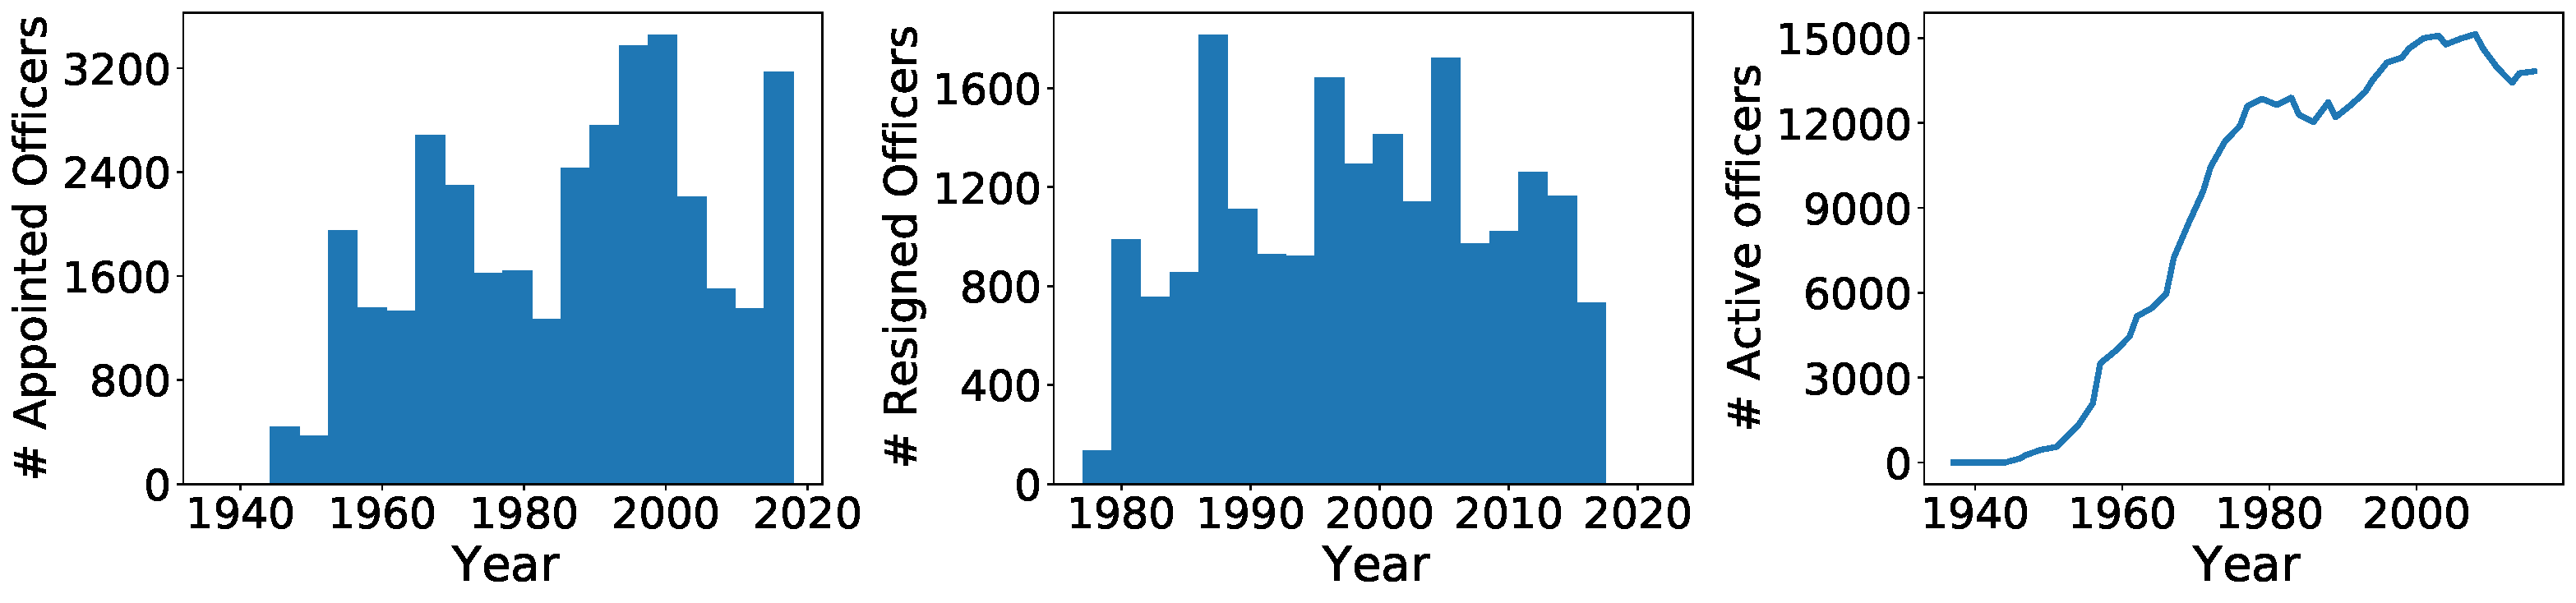
\includegraphics[width=\textwidth]{figs/history} 
\caption{Appointments (left), resignations (center), and the number of active
officers (right) appearing in the CPD roster database from the years 1940 to 2019.}
\label{fig:history}
\end{figure}

\begin{table}[t!]
\caption{Counts of officers (first row) and active officers (resignation date after 2019-01-01, second row). 
Note that ``race'' and ``gender'' are binned per the CPD's coarse categories.} \label{tab:stats}
\begin{tabular}{l|c|c|c|c|c|c|c|c|c|}
\cline{2-3} \cline{5-10}
                                               & \multicolumn{2}{c|}{\textbf{Gender}} & \multicolumn{1}{l|}{} & \multicolumn{6}{c|}{\textbf{Race}}                                                                                                                                                   \\ \cline{2-3} \cline{5-10} 
                                               & {\textbf{M}}   & {\textbf{F}}   &                       & {\textbf{White}} & {\textbf{Black}} & \multicolumn{1}{l|}{{\textbf{Hisp.}}} & {\textbf{Asian/P.I.}} & \multicolumn{1}{l|}{{\textbf{Indig.}}} & {\textbf{Bl. Hisp.}} \\ \cline{1-3} \cline{5-10} 
\multicolumn{1}{|c|}{\textbf{All}}    & 28316                 & 7122                  &                       & 21047                   & 8599                    & 4811                                         & 582                     & 67                                              & 9                           \\ \cline{1-3} \cline{5-10} 
\multicolumn{1}{|c|}{\textbf{Active}} & 11118                 & 4452                  &                       & 7241                    & 3895                    & 3596                                         & 467                     & 40                                              & 9                           \\ \cline{1-3} \cline{5-10} 
\end{tabular} 
\end{table}

\begin{figure}[h] 
	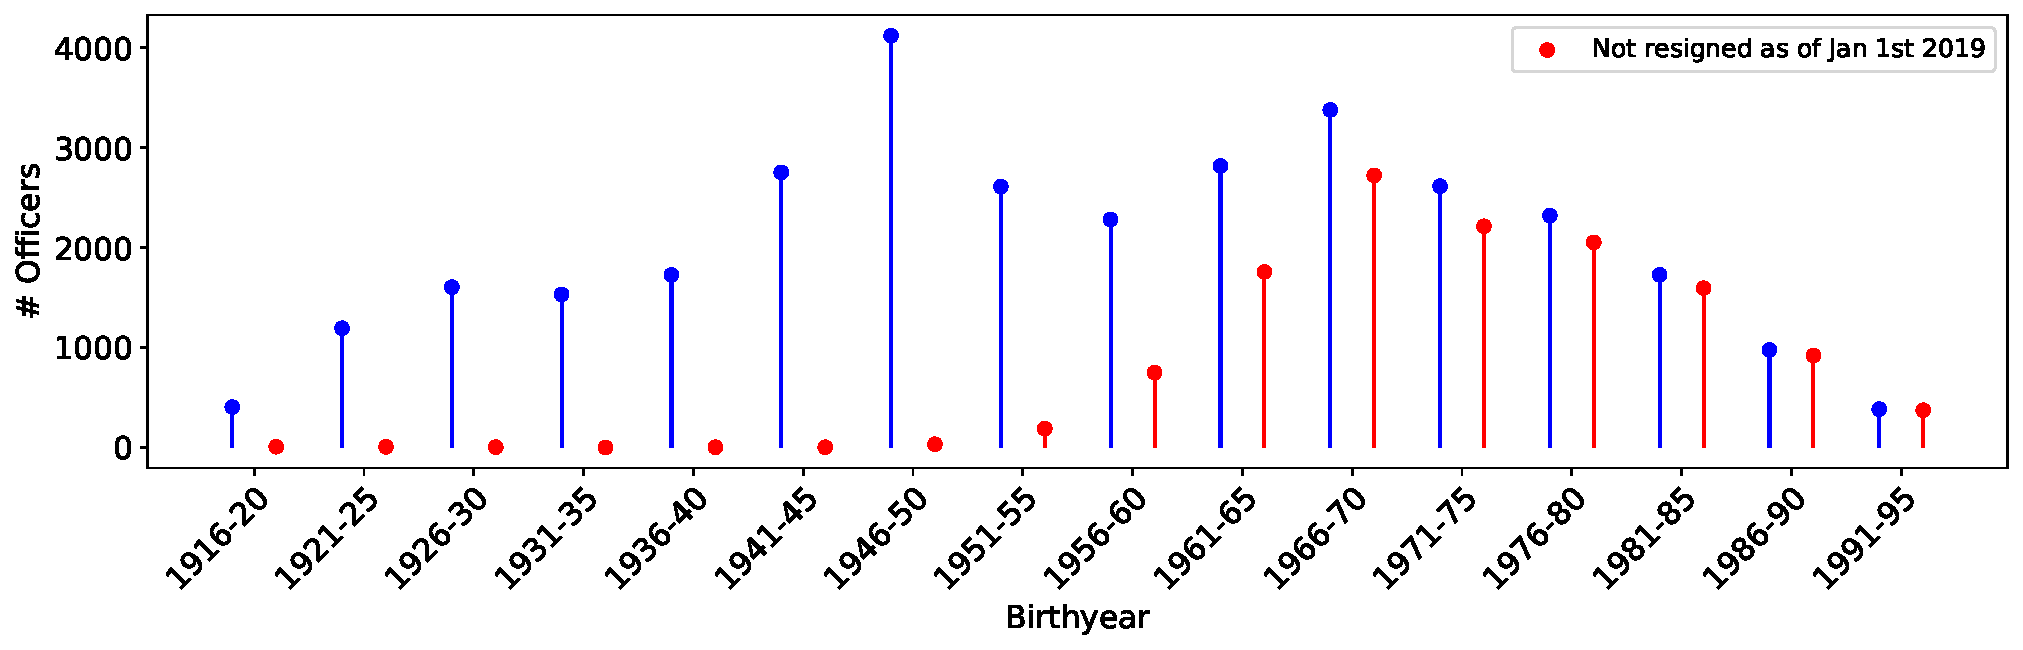
\includegraphics[width=\textwidth]{figs/history_by} 
	\caption{Birthyears for officers in the CPD dataset.} \label{fig:history_by}
\end{figure}

We use the file \texttt{roster.csv} to obtain basic statistics about officers in the CPD dataset. The data contains informations about officers whose appointment dates back to 1936, all the way to 2018 (see \Cref{fig:history}). An important remark to be made is that the data becomes sparser, and less reliable in earlier years. For example, we report in the right subplot of \Cref{fig:history} the number of active officers (vertical axis) as a function of time (horizontal axis): we notice that this number increases sharply between 1940 and 1980. This should be interpreted as a consequence of the lack of data availability for those early years. We also report summary statistics on gender and the CPD race category in \Cref{tab:stats}, and information about officers' birthyears in \Cref{fig:history_by}.

\paragraph{Units.} 
\begin{figure}[h] 
	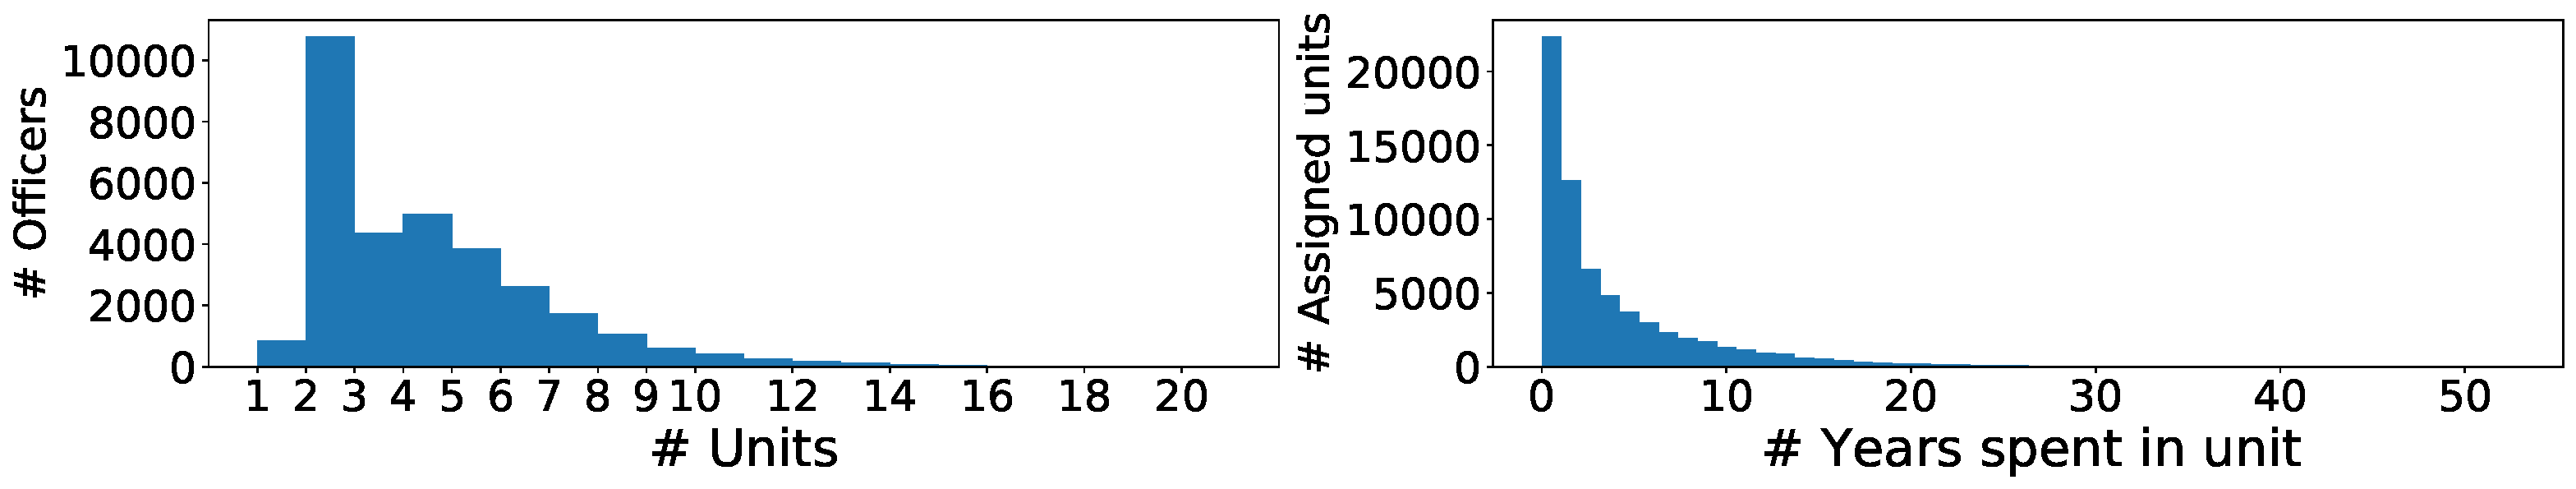
\includegraphics[width=\textwidth]{figs/units_officers} 
	\caption{Histograms of the number of unit assignments for
officers over their career (left), and the number of years spent in each unit for assignments that had terminated by 2019-01-01 (right).}
\label{fig:units}
\end{figure}


We report summary statistics about the number of units an officer is assigned to, and the duration of such appointments in \Cref{fig:units}. The modal number of units appointments is 2: officers typically first joins the acadamy (unit 44), for one or two years, before moving on to a different, often terminal, unit. 
 
\paragraph{Complaints.} 
\begin{figure}[h] 
\begin{subfigure}{0.44\textwidth}
	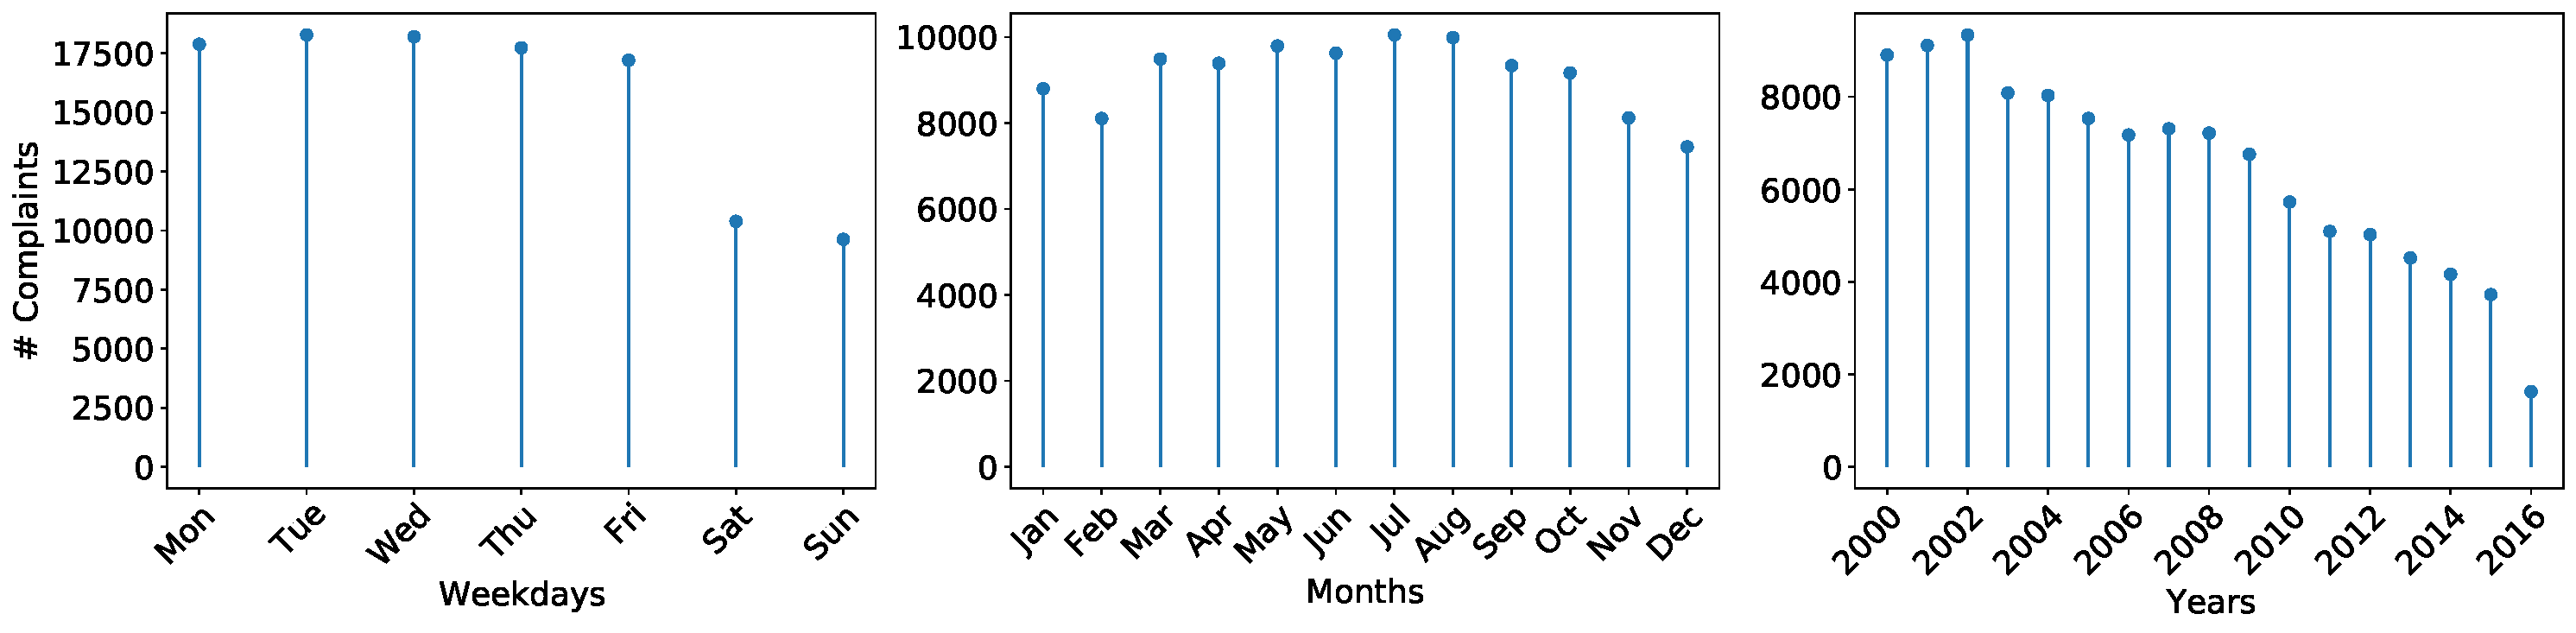
\includegraphics[width=\textwidth, clip, trim= 970 0 0 0]{figs/complaints_times} 
\end{subfigure}
\begin{subfigure}{0.52\textwidth}
	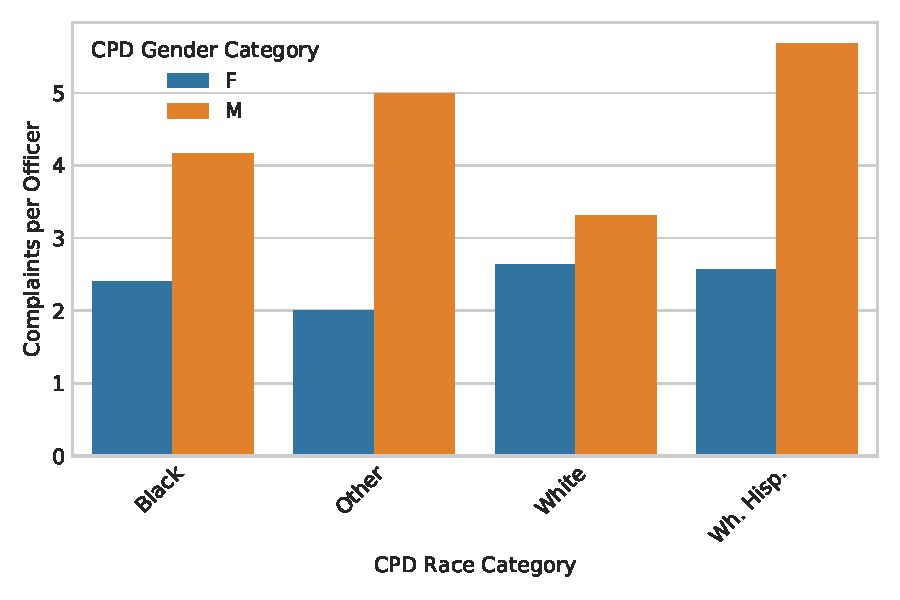
\includegraphics[width=\textwidth]{figs/complaints} 
\end{subfigure}
	\caption{Complaints filed by year (left) and complaints per officer by race and gender (right).} \label{fig:complaints}
\end{figure}

We report in \Cref{fig:complaints} temporal information about complaints filed against the CPD. Interestingly, fewer complaints get filed during the weekends (although, the number of TRRs is higher then --- see \Cref{fig:trrs_times}). Moreover, complaints tend to be higher in the warmer months. Last, we notice that the number of complaints filed kept reducing over the years --- potentially as a consequence of the perception of ineffectiveness of such complaints.

\paragraph{Tactical Response Reports.}

\begin{figure}[h] 
	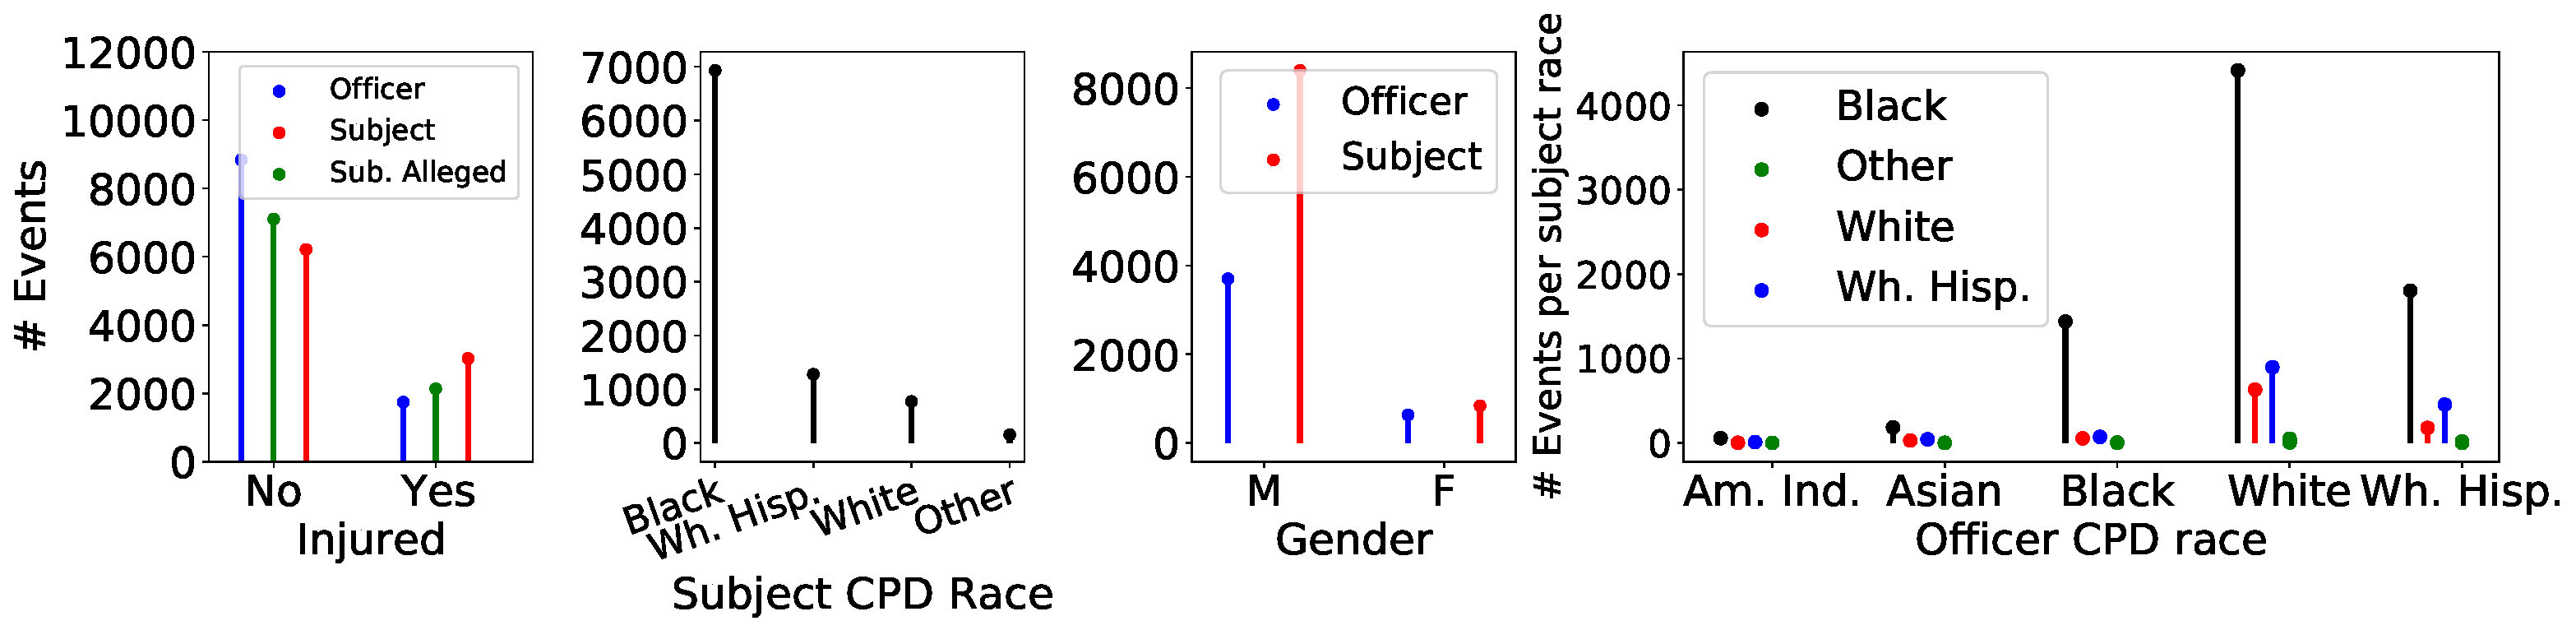
\includegraphics[width=\textwidth]{figs/trr_stats} 
	\caption{Additional statistics for TRRs.} \label{fig:trrs_stats1}
\end{figure}

We also report temporal information about the TRRs in \Cref{fig:trrs_times}. TRRs tend to be filed more frequently at night, in the weekends, and during warmer months. Moreover, 2010, 2011 and 2012 are the years in which the highest number of TRRs have been filed. We also report in \Cref{fig:trrs_stats1} additional information about TRRs: in most cases, neither the officers nor the subjects involved get injured, although civilians get injured at a much higher rate (left subplot), and officers tend to fire first. 
\paragraph{Salary.} todo

\begin{figure}[h] 
\begin{subfigure}{0.4\textwidth}
\raisebox{.5cm}{
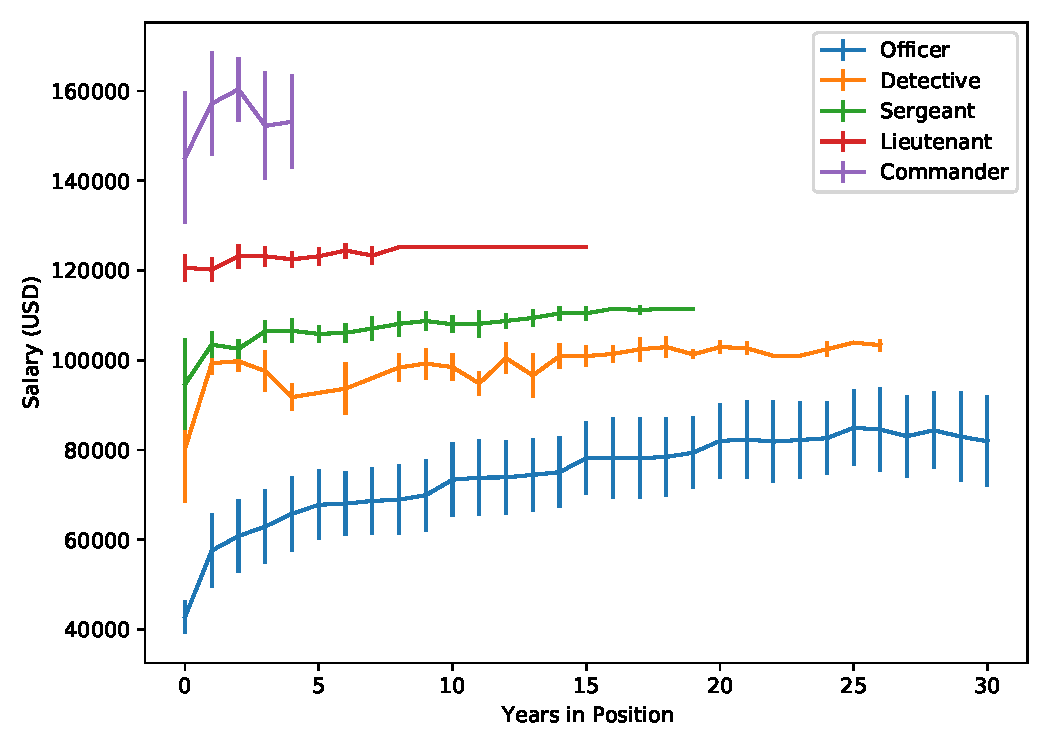
\includegraphics[width=\textwidth]{figs/salary} 
}
\end{subfigure}
\begin{subfigure}{0.5\textwidth}
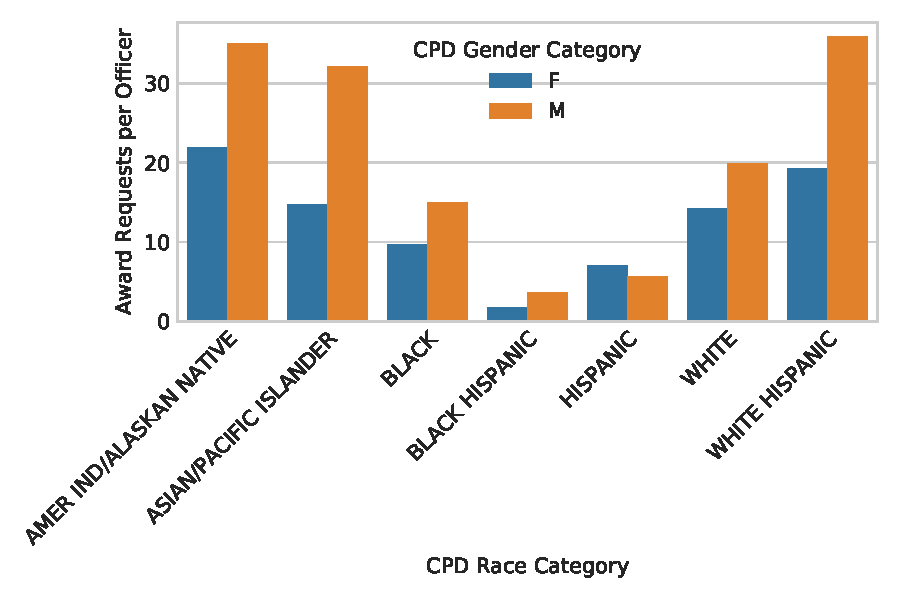
\includegraphics[width=\textwidth]{figs/awards} 
\end{subfigure}
\caption{Historical data from the CPD. Salary versus experience in each
position, years x axis, salary (USD) y axis, for a few of the most common
positions. Lines are means, bars indicate 1 std dev above and below.} \label{fig:salary}
\end{figure}

\paragraph{Awards.}


